\documentclass[12pt,a4paper]{article}

\usepackage[utf8]{inputenc}
\usepackage[spanish]{babel}
\usepackage{graphicx}
\usepackage{geometry}
\geometry{a4paper, margin=2.5cm}
\usepackage{xcolor}
\usepackage{listings}
\usepackage{booktabs}
\usepackage{amsmath}
\usepackage{subcaption}
\usepackage{float}
\usepackage[colorlinks=true, linkcolor=blue, urlcolor=blue]{hyperref}

\definecolor{codegreen}{rgb}{0,0.6,0}
\definecolor{codegray}{rgb}{0.5,0.5,0.5}
\definecolor{codepurple}{rgb}{0.58,0,0.82}
\definecolor{backcolour}{rgb}{0.95,0.95,0.92}

\lstdefinestyle{mystyle}{
    backgroundcolor=\color{backcolour},   
    commentstyle=\color{codegreen},
    keywordstyle=\color{magenta},
    numberstyle=\tiny\color{codegray},
    stringstyle=\color{codepurple},
    basicstyle=\ttfamily\footnotesize,
    breakatwhitespace=false,         
    breaklines=true,                 
    captionpos=b,                    
    keepspaces=true,                 
    numbers=left,                    
    numbersep=5pt,                  
    showspaces=false,                
    showstringspaces=false,
    showtabs=false,                  
    tabsize=2,
    literate={á}{{\'a}}1 {é}{{\'e}}1 {í}{{\'i}}1 {ó}{{\'o}}1 {ú}{{\'u}}1
             {Á}{{\'A}}1 {É}{{\'E}}1 {Í}{{\'I}}1 {Ó}{{\'O}}1 {Ú}{{\'U}}1
             {ñ}{{\~n}}1 {Ñ}{{\~N}}1
}
\lstset{style=mystyle}

\title{\Huge\textbf{PROYECTO ESP32} \\ \Large Control de Brillo de LED con Potenciómetro y Bluetooth \\ \vspace{0.5cm} \normalsize \textit{Lectura analógica ADC, modulación PWM y transmisión inalámbrica de datos vía Bluetooth Classic}}
\author{Msc. Néstor Fabio Montoya Palacios}
\date{2026 \\ \vspace{0.2cm} \small Plataforma: ESP32 Dev Module}

\begin{document}

\maketitle
\tableofcontents
\newpage

% ══════════════════════════════════════════════════════════════
\section{Introducción}
% ══════════════════════════════════════════════════════════════

Este documento describe de manera detallada el proyecto ``Control de Brillo de LED con Potenciómetro y Bluetooth'', una extensión del proyecto básico de potenciómetro que incorpora \textbf{comunicación inalámbrica Bluetooth Classic} mediante el perfil SPP (\textit{Serial Port Profile}) del ESP32. El sistema lee la posición angular de un potenciómetro mediante el ADC del ESP32, controla el brillo de un LED proporcionalmente mediante PWM, y \textbf{transmite los datos en tiempo real a un dispositivo móvil} a través de Bluetooth, utilizando la aplicación \textit{Serial Bluetooth Terminal}.

Este proyecto añade una capa de comunicación inalámbrica al control analógico-digital básico, permitiendo al usuario monitorear remotamente los valores del sensor desde un teléfono celular sin necesidad de estar conectado físicamente al computador. Se introducen los conceptos de \textbf{Bluetooth Classic SPP}, la librería \texttt{BluetoothSerial.h} del ESP32, y la \textbf{transmisión dual} de datos (simultáneamente por USB serial y por Bluetooth).

% ══════════════════════════════════════════════════════════════
\section{Objetivo del Proyecto}
% ══════════════════════════════════════════════════════════════

Implementar un sistema de control analógico-digital con monitoreo inalámbrico utilizando el ESP32 que:
\begin{itemize}
    \item Lea la posición de un potenciómetro mediante el ADC de 12 bits (rango 0--4095).
    \item Convierta los valores digitales a voltaje (rango 0--3,3\,V).
    \item Controle proporcionalmente el brillo de un LED mediante PWM de 8 bits.
    \item Transmita los datos simultáneamente por \textbf{USB Serial} (al computador) y por \textbf{Bluetooth Serial} (al celular).
    \item Permita la conexión inalámbrica desde la aplicación \textit{Serial Bluetooth Terminal} usando el nombre de dispositivo ``EQUIPO\_MARAVILLA''.
\end{itemize}

% ══════════════════════════════════════════════════════════════
\section{Materiales Necesarios}
% ══════════════════════════════════════════════════════════════

\begin{table}[h!]
\centering
\begin{tabular}{cll}
\toprule
\textbf{Cant.} & \textbf{Componente} & \textbf{Especificación} \\
\midrule
1 & ESP32 Dev Module & Microcontrolador dual-core con Wi-Fi/Bluetooth \\
1 & Potenciómetro & 10\,k$\Omega$ lineal, 3 terminales \\
1 & LED & Diodo emisor de luz, 5\,mm \\
1 & Resistencia & 220\,$\Omega$ (limitadora de corriente) \\
1 & Protoboard & Placa de pruebas de 830 puntos \\
  & Cables jumper & Macho-macho para conexiones \\
1 & Cable USB & Para programación y alimentación \\
1 & Teléfono celular & Con Bluetooth y app Serial Bluetooth Terminal \\
\bottomrule
\end{tabular}
\caption{Lista de materiales del proyecto Potenciómetro con Bluetooth}
\end{table}

% ══════════════════════════════════════════════════════════════
\section{Esquema de Conexión}
% ══════════════════════════════════════════════════════════════

El circuito utiliza el mismo esquema de conexión que el proyecto básico de potenciómetro. El potenciómetro se conecta como divisor de voltaje entre 3,3\,V y GND, con su cursor en GPIO34. El LED se conecta a GPIO4 mediante una resistencia de 220\,$\Omega$. La comunicación Bluetooth no requiere hardware adicional, ya que el ESP32 integra el módulo de radio en el propio chip.

\begin{figure}[H]
\centering
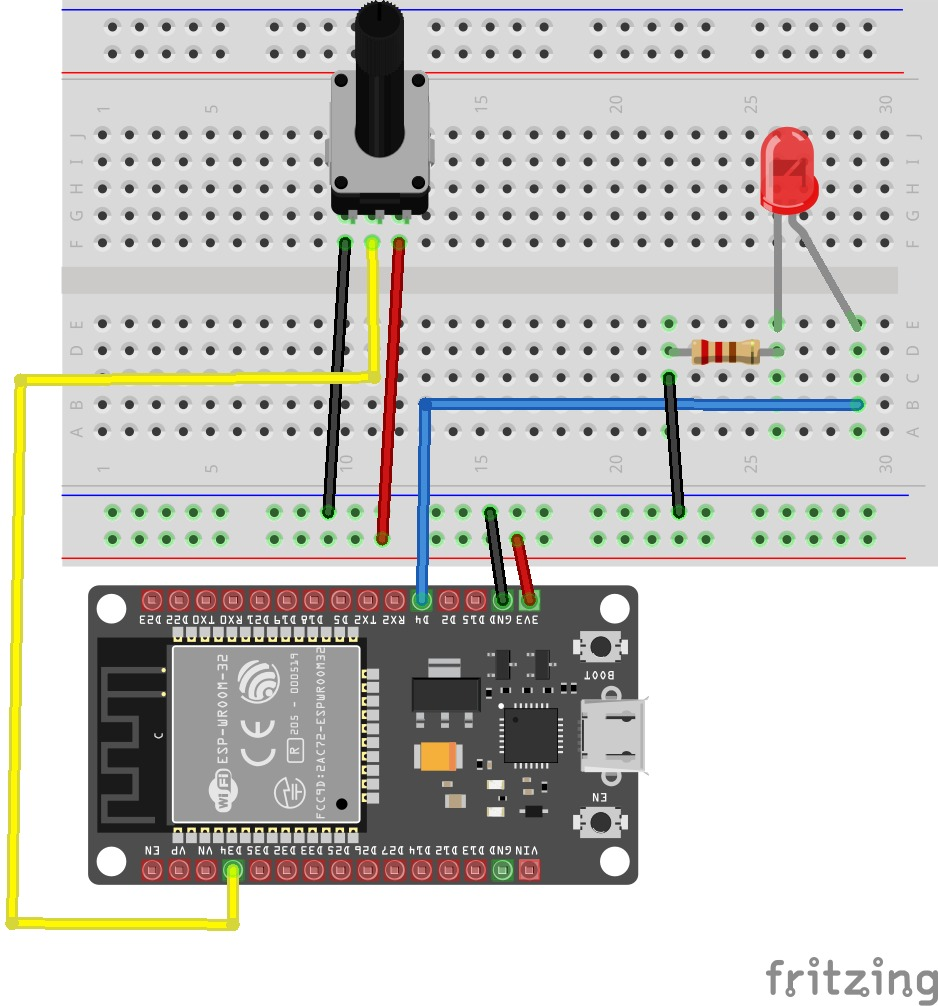
\includegraphics[width=0.85\textwidth]{../Esquemas/Potenciometro_esq.jpeg}
\caption{Esquema de conexión del circuito en Fritzing -- el Bluetooth es interno al ESP32}
\label{fig:esquema}
\end{figure}

\subsection{Diagrama de Conexiones}

\begin{center}
\begin{tabular}{lll}
\toprule
\textbf{Componente} & \textbf{Pin} & \textbf{ESP32 GPIO} \\
\midrule
Potenciómetro & Terminal 1 & 3.3V \\
Potenciómetro & Terminal 2 (cursor) & GPIO34 (ADC1\_CH6) \\
Potenciómetro & Terminal 3 & GND \\
Resistencia 220\,$\Omega$ & Terminal 1 & GPIO4 \\
LED & Ánodo (+) & Resistencia 220\,$\Omega$ (Terminal 2) \\
LED & Cátodo (--) & GND \\
\bottomrule
\end{tabular}
\end{center}

\textbf{Nota importante:} A diferencia de módulos Bluetooth externos (como el HC-05), el ESP32 integra el controlador Bluetooth directamente en su SoC, por lo que \textbf{no se requieren conexiones adicionales} para la funcionalidad inalámbrica. El módulo de radio comparte la antena PCB impresa en la placa de desarrollo.

% ══════════════════════════════════════════════════════════════
\section{Código Fuente}
% ══════════════════════════════════════════════════════════════

A continuación se presenta el código completo del proyecto. Respecto al proyecto básico de potenciómetro, se añade la librería \texttt{BluetoothSerial.h} y el envío paralelo de datos por Bluetooth.

\subsection{Código Completo}
\lstinputlisting[language=C++, title=Potenciometro\_Bluetooth.ino]{../Arduino/Potenciometro_Bluetooth/Potenciometro_Bluetooth.ino}

% ══════════════════════════════════════════════════════════════
\subsection{Análisis del Código}
% ══════════════════════════════════════════════════════════════

\subsubsection*{Inclusión de la Librería Bluetooth}
El programa comienza incluyendo la librería \texttt{BluetoothSerial.h}, que forma parte del Arduino Core para ESP32 y proporciona una interfaz de comunicación serie sobre Bluetooth Classic (perfil SPP). Se crea una instancia global del objeto \texttt{BluetoothSerial} llamada \texttt{BT}, que se utilizará para enviar y recibir datos de forma inalámbrica.

\subsubsection*{Declaración de Pines y Constantes}
\begin{itemize}
    \item \textbf{\texttt{pinPotenciometro = 34}:} GPIO34, entrada analógica ADC1\_CH6 (pin de solo entrada).
    \item \textbf{\texttt{pinLED = 4}:} GPIO4, salida PWM para el LED.
    \item \textbf{\texttt{frecuenciaPWM = 5000}:} Frecuencia PWM de 5\,kHz.
    \item \textbf{\texttt{resolucionPWM = 8}:} 256 niveles de brillo (0--255).
\end{itemize}

\subsubsection*{Función \texttt{setup()}}
\begin{enumerate}
    \item Inicia la comunicación serial USB a 115200 baudios.
    \item \textbf{Inicia el Bluetooth} con \texttt{BT.begin("EQUIPO\_MARAVILLA")}, haciendo visible el ESP32 como dispositivo Bluetooth con ese nombre.
    \item Configura GPIO34 como entrada analógica.
    \item Configura el canal PWM en GPIO4 con \texttt{ledcAttach()}.
    \item Imprime mensajes de bienvenida indicando que el Bluetooth está listo.
\end{enumerate}

\subsubsection*{Función \texttt{loop()}}
El bucle principal ejecuta siete pasos en cada iteración:

\begin{enumerate}
    \item \textbf{PASO 1 -- Lectura analógica:} \texttt{analogRead()} lee el potenciómetro (0--4095).
    \item \textbf{PASO 2 -- Conversión a voltaje:}
    \begin{equation}
    V = \frac{\text{valor} \times 3{,}3}{4095}
    \label{eq:voltaje}
    \end{equation}
    \item \textbf{PASO 3 -- Mapeo a brillo PWM:} \texttt{map(valor, 0, 4095, 0, 255)}.
    \item \textbf{PASO 4 -- Escritura PWM:} \texttt{ledcWrite(pinLED, brillo)}.
    \item \textbf{PASO 5 -- Construcción del mensaje:} Se concatena un \texttt{String} con valor ADC, voltaje y brillo.
    \item \textbf{PASO 6 -- Envío por USB Serial:} \texttt{Serial.println(mensaje)}.
    \item \textbf{PASO 7 -- Envío por Bluetooth:} \texttt{BT.println(mensaje)} transmite los mismos datos al celular.
\end{enumerate}

El ciclo se repite cada 300\,ms.

% ══════════════════════════════════════════════════════════════
\section{Principio de Funcionamiento}
% ══════════════════════════════════════════════════════════════

\subsection{Bluetooth Classic en el ESP32}

El ESP32 integra un controlador Bluetooth dual-mode que soporta tanto \textbf{Bluetooth Classic} (BR/EDR) como \textbf{Bluetooth Low Energy} (BLE). En este proyecto se utiliza Bluetooth Classic con el perfil \textbf{SPP} (\textit{Serial Port Profile}), que emula un puerto serial inalámbrico.

La librería \texttt{BluetoothSerial.h} encapsula toda la complejidad del stack Bluetooth, proporcionando una API idéntica a la clase \texttt{Serial}:

\begin{itemize}
    \item \texttt{BT.begin("nombre")}: Inicializa el stack Bluetooth y hace visible el dispositivo.
    \item \texttt{BT.println(dato)}: Envía datos como texto seguido de salto de línea.
    \item \texttt{BT.available()}: Verifica si hay datos recibidos (no usado en este proyecto).
    \item \texttt{BT.read()}: Lee un byte recibido (no usado en este proyecto).
\end{itemize}

El proceso de conexión desde el celular es:
\begin{enumerate}
    \item Activar Bluetooth en el teléfono.
    \item Emparejar con el dispositivo ``EQUIPO\_MARAVILLA''.
    \item Abrir la app \textit{Serial Bluetooth Terminal} y conectar al dispositivo emparejado.
    \item Los datos del potenciómetro aparecen en pantalla en tiempo real.
\end{enumerate}

\subsection{Transmisión Dual de Datos}

Una característica importante de este proyecto es la \textbf{transmisión dual}: los mismos datos se envían simultáneamente por dos canales independientes:

\begin{center}
\begin{tabular}{lll}
\toprule
\textbf{Canal} & \textbf{Función} & \textbf{Receptor} \\
\midrule
USB Serial & \texttt{Serial.println()} & Monitor Serial del Arduino IDE \\
Bluetooth SPP & \texttt{BT.println()} & App Serial Bluetooth Terminal \\
\bottomrule
\end{tabular}
\end{center}

Esto permite depurar el sistema desde el computador mientras el usuario final monitorea los datos desde el celular.

\subsection{Cadena de Procesamiento}

\begin{verbatim}
    Potenciómetro        ADC 12-bit       Mapeo         PWM 8-bit
    (ángulo)    ─────>  (0 - 4095)  ─────> map() ─────> (0 - 255)
    0° - 270°            voltaje           brillo        duty cycle
                        0 - 3.3 V                       0% - 100%
                                                           │
                              ┌────────────────────────────┤
                              v                            v
                        Bluetooth SPP              Brillo del LED
                     (al celular vía app)
                              │
                              v
                        USB Serial
                  (al monitor del Arduino IDE)
\end{verbatim}

\subsection{El Potenciómetro como Divisor de Voltaje}

El potenciómetro actúa como divisor de voltaje ajustable. Con sus terminales extremos entre 3,3\,V y GND:

\begin{equation}
V_{\text{cursor}} = V_{CC} \times \frac{\theta}{\theta_{\max}} = 3{,}3 \times \frac{\theta}{270°}
\label{eq:divisor}
\end{equation}

\subsection{Modulación por Ancho de Pulso (PWM)}

El ciclo de trabajo controla el brillo percibido del LED:
\begin{equation}
D = \frac{t_{\text{ON}}}{T} \times 100\,\%
\label{eq:duty}
\end{equation}

Con 8 bits de resolución y 5\,kHz de frecuencia ($T = 200\,\mu$s), se obtienen 256 niveles de brillo sin parpadeo visible.

% ══════════════════════════════════════════════════════════════
\section{Fotografías del Montaje}
% ══════════════════════════════════════════════════════════════

Las siguientes imágenes documentan el proyecto en funcionamiento, mostrando el montaje físico, la recepción de datos en el celular vía Bluetooth, y el entorno de desarrollo Arduino IDE.

\begin{figure}[H]
\centering
\begin{subfigure}[b]{0.48\textwidth}
    \centering
    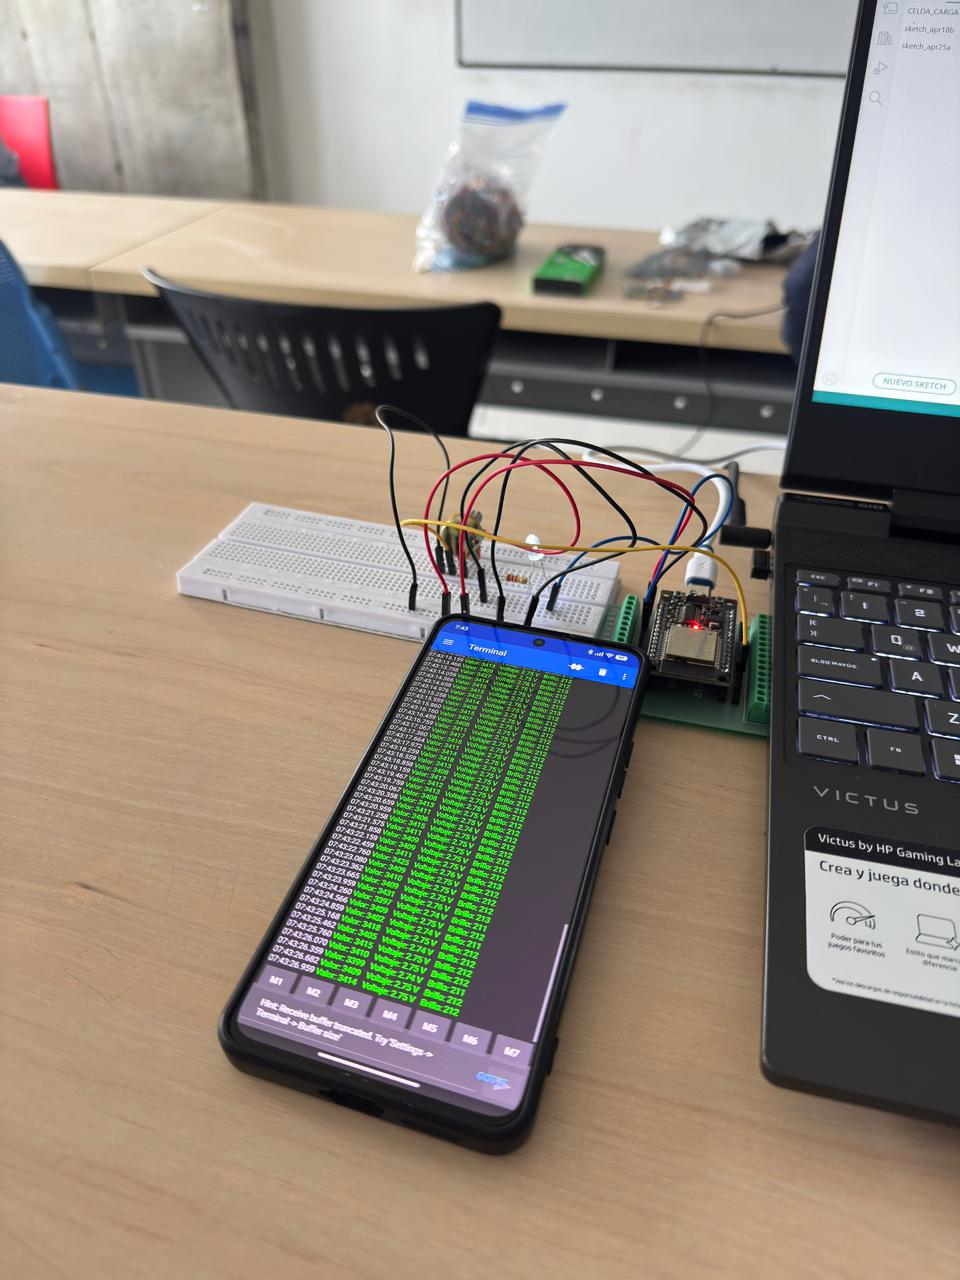
\includegraphics[width=\textwidth]{../Imagenes/Potenciometro_bluetoot_imgs/Potenciometro_bluetooth_img1.jpeg}
    \caption{Vista general: celular recibiendo datos por Bluetooth, ESP32 en placa de expansión y protoboard con el circuito}
    \label{fig:bt1}
\end{subfigure}
\hfill
\begin{subfigure}[b]{0.48\textwidth}
    \centering
    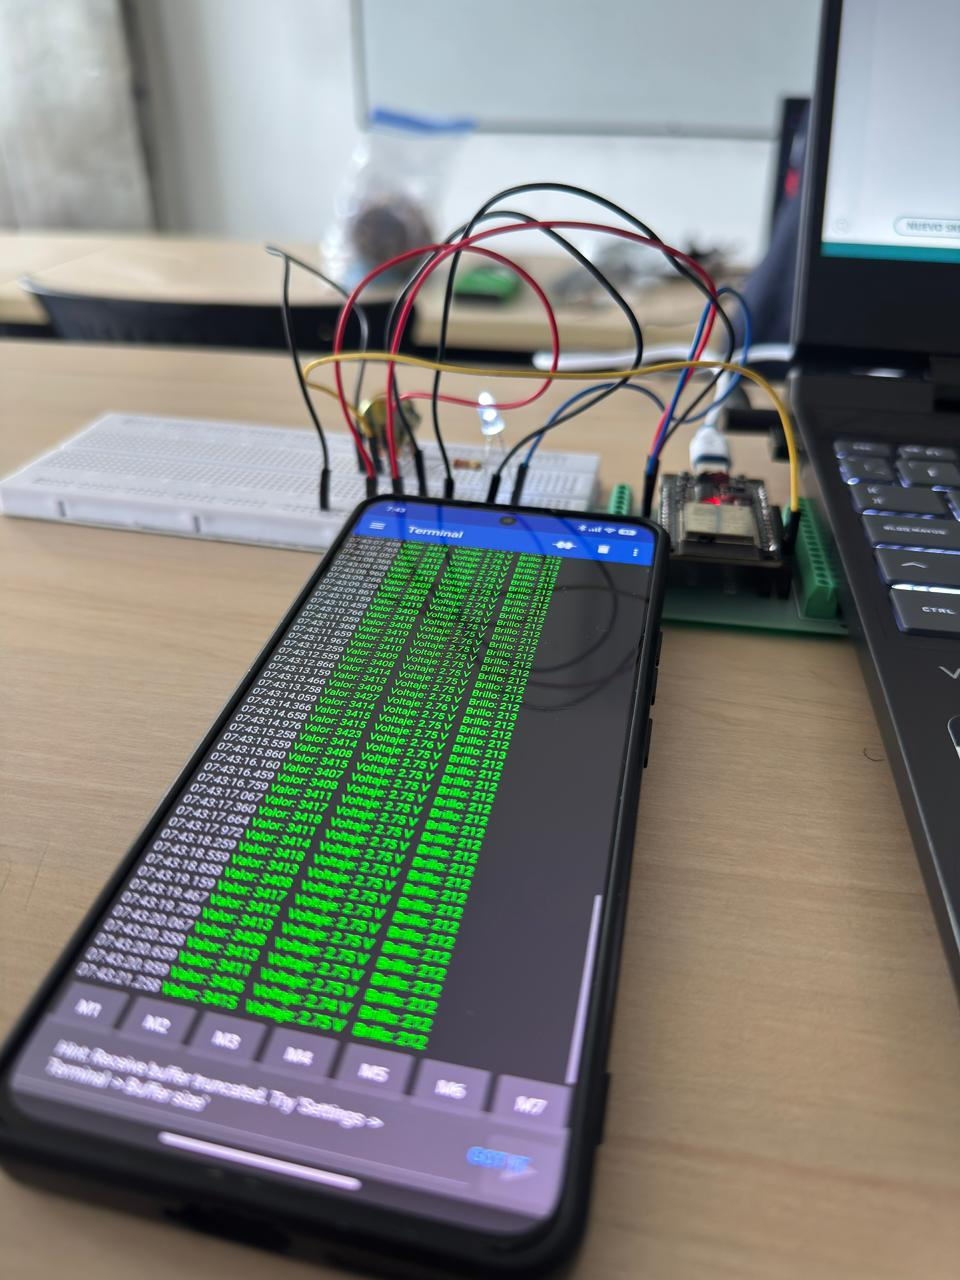
\includegraphics[width=\textwidth]{../Imagenes/Potenciometro_bluetoot_imgs/Potenciometro_bluetooth_img2.jpeg}
    \caption{Detalle de la app Serial Bluetooth Terminal mostrando valores de ADC, voltaje y brillo en tiempo real}
    \label{fig:bt2}
\end{subfigure}
\caption{Montaje y recepción de datos Bluetooth}
\label{fig:montaje1}
\end{figure}

\begin{figure}[H]
\centering
\begin{subfigure}[b]{0.48\textwidth}
    \centering
    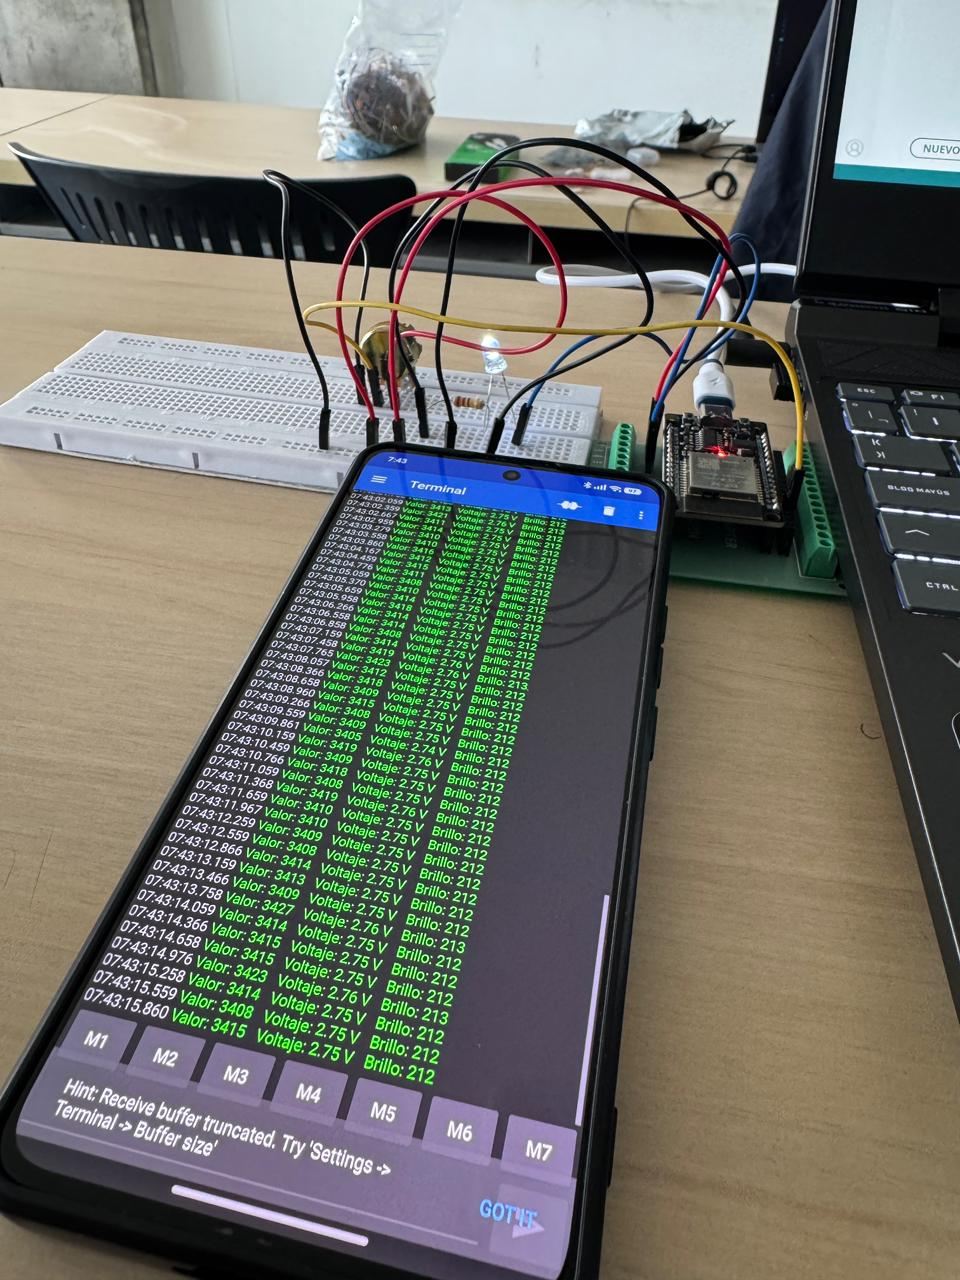
\includegraphics[width=\textwidth]{../Imagenes/Potenciometro_bluetoot_imgs/Potenciometro_bluetooth_img3.jpeg}
    \caption{Vista detallada de la terminal Bluetooth con timestamps y datos legibles del potenciómetro}
    \label{fig:bt3}
\end{subfigure}
\hfill
\begin{subfigure}[b]{0.48\textwidth}
    \centering
    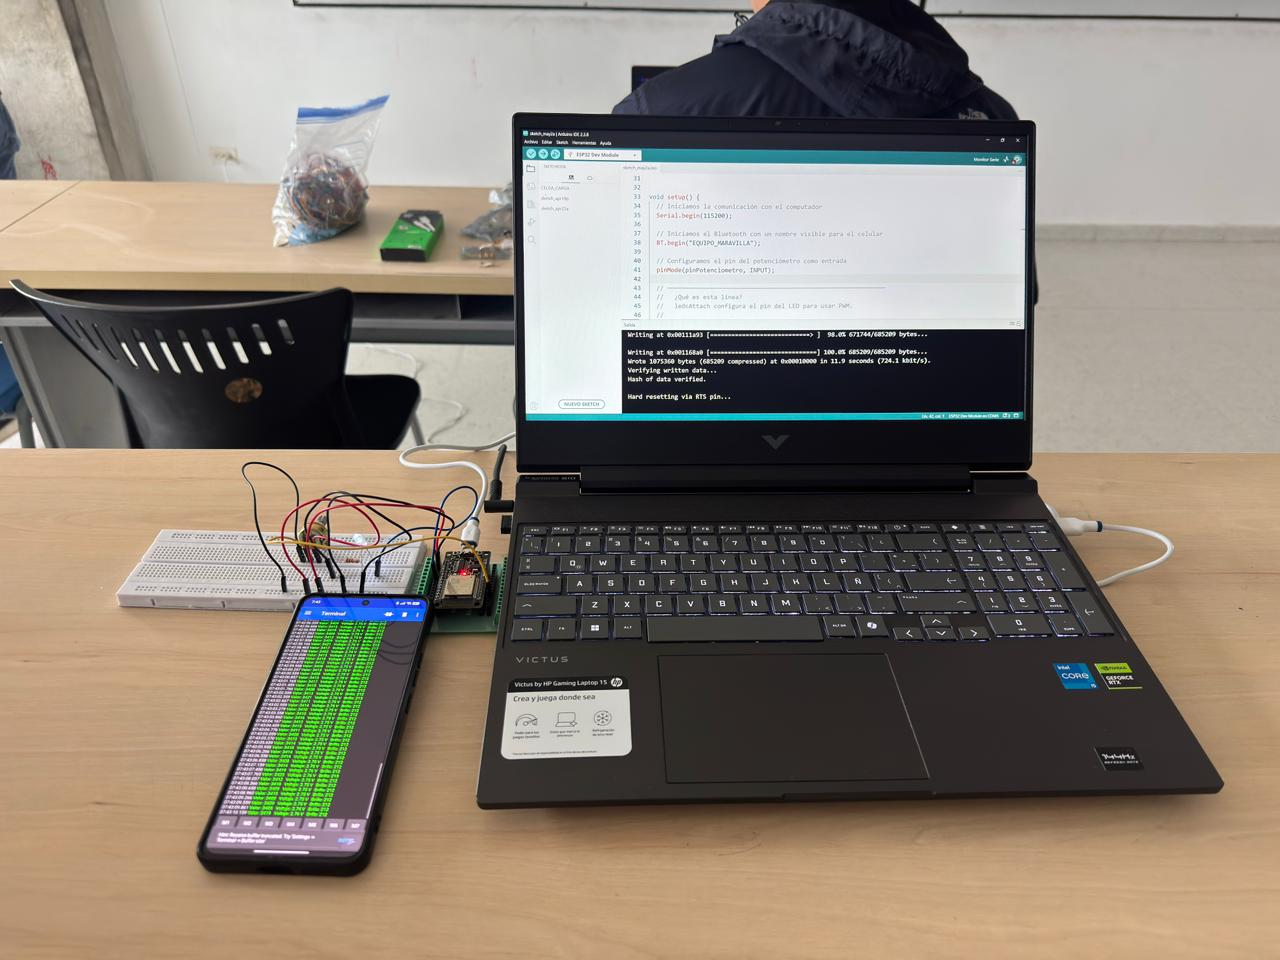
\includegraphics[width=\textwidth]{../Imagenes/Potenciometro_bluetoot_imgs/Potenciometro_bluetooth_img4.jpeg}
    \caption{Arduino IDE con el código fuente y la consola mostrando la carga exitosa del firmware al ESP32}
    \label{fig:bt4}
\end{subfigure}
\caption{Terminal Bluetooth y entorno de desarrollo}
\label{fig:montaje2}
\end{figure}

\begin{figure}[H]
\centering
\begin{subfigure}[b]{0.48\textwidth}
    \centering
    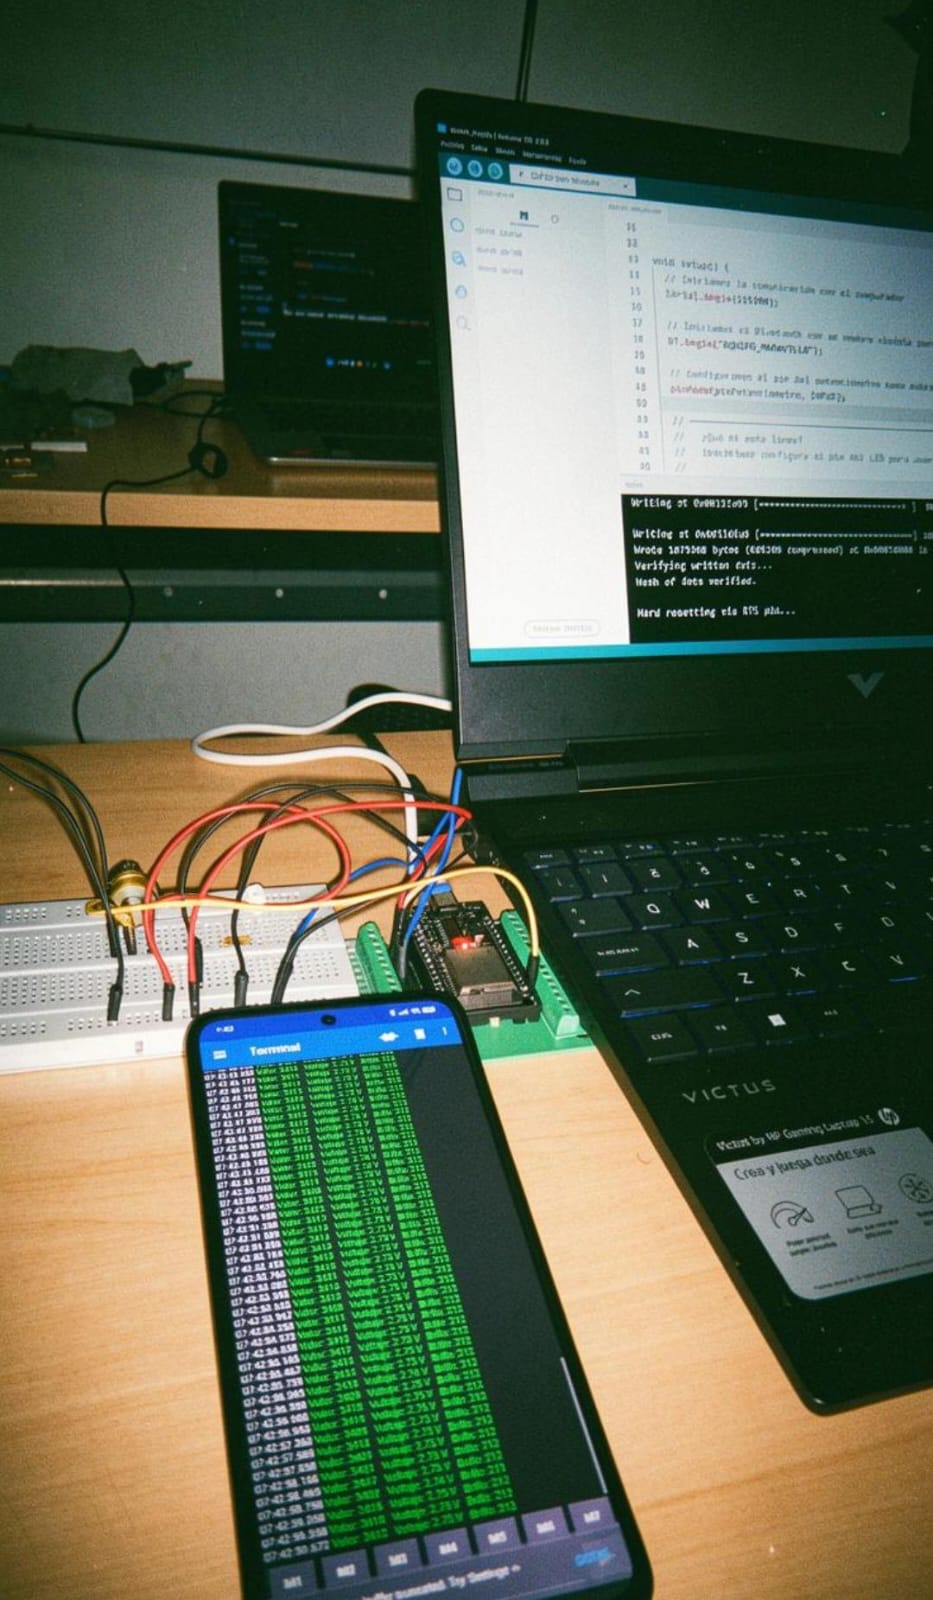
\includegraphics[width=\textwidth]{../Imagenes/Potenciometro_bluetoot_imgs/Potenciometro_bluetooth_img5.jpeg}
    \caption{Vista alternativa del setup completo: laptop con Arduino IDE, celular con terminal Bluetooth y circuito en protoboard}
    \label{fig:bt5}
\end{subfigure}
\hfill
\begin{subfigure}[b]{0.48\textwidth}
    \centering
    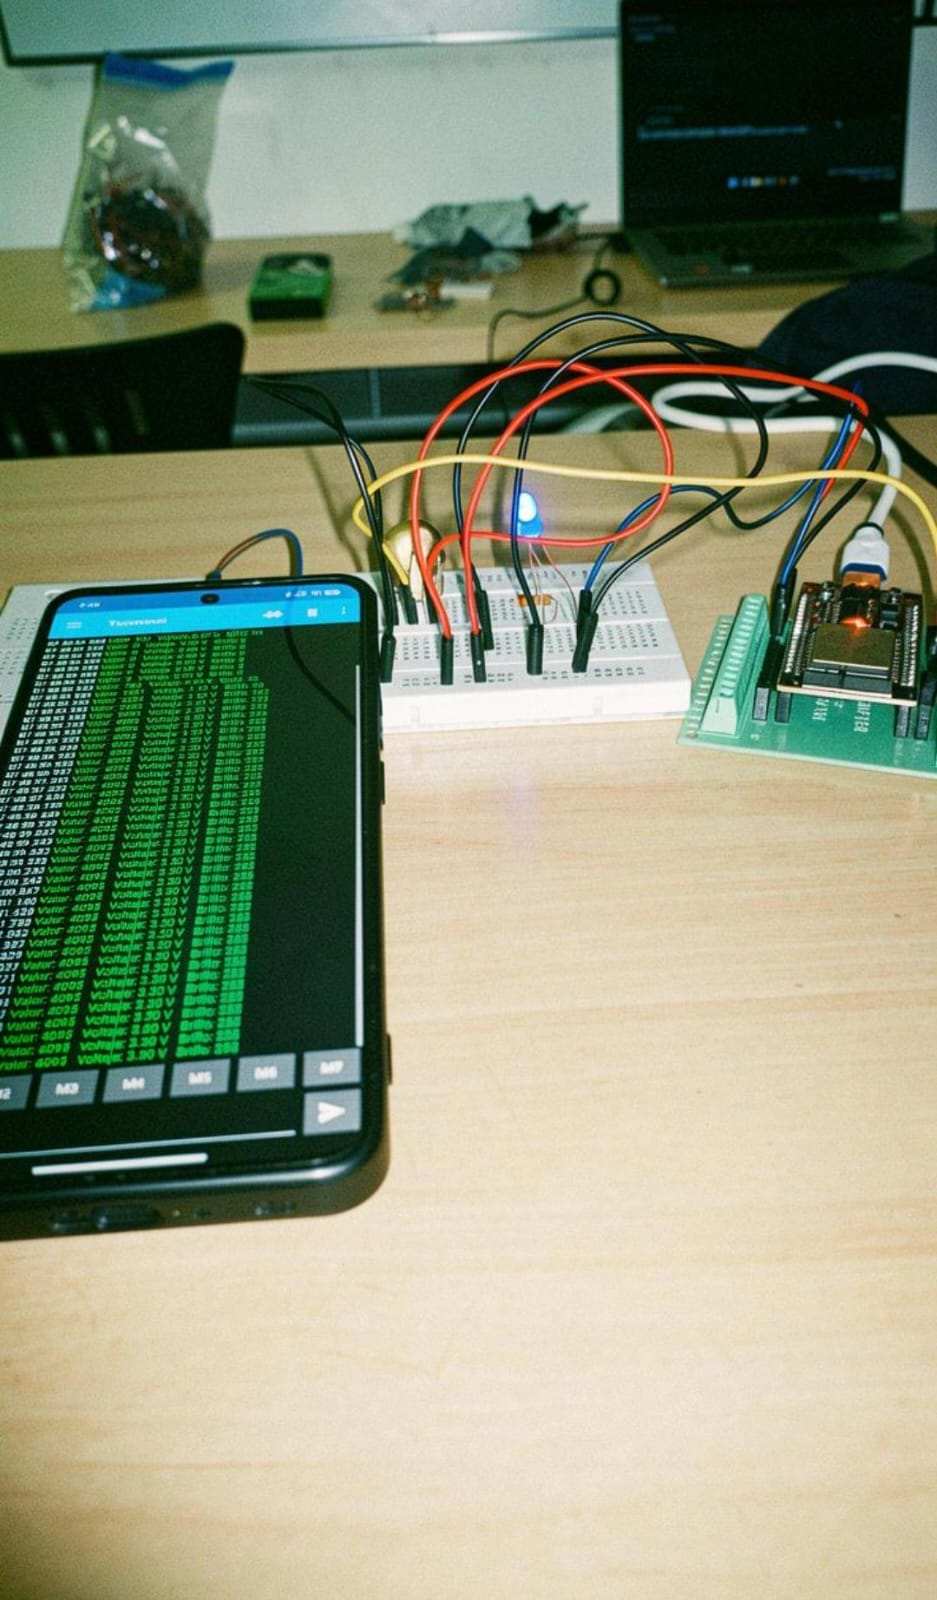
\includegraphics[width=\textwidth]{../Imagenes/Potenciometro_bluetoot_imgs/Potenciometro_bluetooth_img6.jpeg}
    \caption{LED encendido con brillo controlado por el potenciómetro mientras el celular recibe datos inalámbricamente}
    \label{fig:bt6}
\end{subfigure}
\caption{Vistas adicionales del proyecto en funcionamiento}
\label{fig:montaje3}
\end{figure}

En las Figuras~\ref{fig:bt1} a~\ref{fig:bt6} se puede observar:
\begin{itemize}
    \item La app \textit{Serial Bluetooth Terminal} muestra datos con formato \texttt{Valor: XXXX  Voltaje: X.XX V  Brillo: XXX} con timestamps.
    \item Los valores típicos observados rondan \texttt{Valor: 3410}, \texttt{Voltaje: 2.75 V}, \texttt{Brillo: 212}, indicando que el potenciómetro se encuentra en una posición cercana al 83\% de su recorrido.
    \item El LED se observa encendido con brillo correspondiente al ciclo de trabajo PWM.
    \item La consola del Arduino IDE confirma la carga exitosa del firmware: ``Hash of data verified. Hard resetting via RTS pin...''.
\end{itemize}

% ══════════════════════════════════════════════════════════════
\section{Videos de Funcionamiento}
% ══════════════════════════════════════════════════════════════

Se dispone de dos videos que demuestran el funcionamiento del proyecto:

\begin{itemize}
    \item \textbf{Potenciometro\_bluetooth\_Funcionamiento1.mp4}: Demostración completa del sistema, mostrando la variación del brillo del LED al girar el potenciómetro y la recepción simultánea de datos en el celular vía Bluetooth.
    \item \textbf{Potenciometro\_bluetooth\_Funcionamiento2.mp4}: Demostración enfocada en la transmisión Bluetooth, mostrando la actualización en tiempo real de los valores en la app Serial Bluetooth Terminal.
\end{itemize}

Estos videos se encuentran en la carpeta \texttt{Videos/Potenciometro\_bluetooth\_vid/} del repositorio del proyecto.

% ══════════════════════════════════════════════════════════════
\section{Proceso de Creación}
% ══════════════════════════════════════════════════════════════

El desarrollo de este proyecto partió del proyecto base de potenciómetro y añadió la funcionalidad Bluetooth siguiendo estos pasos:

\begin{enumerate}
    \item \textbf{Punto de partida:} Se tomó como base el proyecto ``Control de LED con Potenciómetro'' (sin Bluetooth), que ya implementaba la lectura ADC, conversión a voltaje y control PWM del LED.
    
    \item \textbf{Incorporación de la librería Bluetooth:} Se añadió \texttt{\#include "BluetoothSerial.h"} y se creó la instancia \texttt{BluetoothSerial BT}, que proporciona la interfaz de comunicación inalámbrica.
    
    \item \textbf{Inicialización del Bluetooth:} En \texttt{setup()}, se añadió \texttt{BT.begin("EQUIPO\_MARAVILLA")} para inicializar el stack Bluetooth Classic con un nombre identificable para el emparejamiento desde el celular.
    
    \item \textbf{Transmisión dual de datos:} En \texttt{loop()}, se añadió \texttt{BT.println(mensaje)} después de \texttt{Serial.println(mensaje)}, enviando los mismos datos por ambos canales simultáneamente.
    
    \item \textbf{Preparación del celular:}
    \begin{itemize}
        \item Se instaló la app \textit{Serial Bluetooth Terminal} desde Google Play Store.
        \item Se emparejó el celular con ``EQUIPO\_MARAVILLA'' desde la configuración de Bluetooth.
        \item Se estableció la conexión desde la app para recibir datos.
    \end{itemize}
    
    \item \textbf{Configuración del Arduino IDE:}
    \begin{itemize}
        \item Placa: \textit{ESP32 Dev Module}.
        \item Velocidad de subida: 115200 baudios.
        \item Puerto COM correspondiente al ESP32.
    \end{itemize}
    
    \item \textbf{Pruebas y validación:} Se verificó que los datos aparecieran correctamente tanto en el monitor serial del computador como en la app del celular, y que el brillo del LED respondiera proporcionalmente al potenciómetro.
\end{enumerate}

% ══════════════════════════════════════════════════════════════
\section{Diferencias con el Proyecto Base}
% ══════════════════════════════════════════════════════════════

\begin{table}[H]
\centering
\begin{tabular}{lcc}
\toprule
\textbf{Característica} & \textbf{Proyecto Base} & \textbf{Con Bluetooth} \\
\midrule
Lectura ADC & \checkmark & \checkmark \\
Conversión a voltaje & \checkmark & \checkmark \\
Control PWM del LED & \checkmark & \checkmark \\
Monitoreo USB Serial & \checkmark & \checkmark \\
Comunicación Bluetooth & -- & \checkmark \\
Monitoreo desde celular & -- & \checkmark \\
Librería BluetoothSerial & -- & \checkmark \\
Hardware adicional requerido & -- & Ninguno \\
\bottomrule
\end{tabular}
\caption{Comparación entre el proyecto base y la versión con Bluetooth}
\end{table}

% ══════════════════════════════════════════════════════════════
\section{Conceptos Técnicos Clave}
% ══════════════════════════════════════════════════════════════

\subsection{Bluetooth Classic vs BLE}

\begin{table}[H]
\centering
\begin{tabular}{lll}
\toprule
\textbf{Característica} & \textbf{Bluetooth Classic} & \textbf{BLE} \\
\midrule
Perfil usado & SPP (Serial Port) & GATT \\
Velocidad & Hasta 3 Mbps & Hasta 1 Mbps \\
Consumo & Mayor & Menor \\
Alcance típico & 10--100 m & 10--100 m \\
Complejidad & Menor (API Serial) & Mayor (servicios/características) \\
Uso en este proyecto & \checkmark & -- \\
\bottomrule
\end{tabular}
\caption{Comparación Bluetooth Classic vs BLE}
\end{table}

En este proyecto se eligió Bluetooth Classic por su simplicidad: la API de \texttt{BluetoothSerial} replica exactamente el comportamiento de \texttt{Serial}, lo que minimiza los cambios en el código respecto al proyecto base.

\subsection{La Librería BluetoothSerial.h}

Esta librería forma parte del Arduino Core para ESP32 y encapsula el stack Bluetooth Classic. Sus funciones principales son:

\begin{itemize}
    \item \texttt{begin(nombre)}: Inicializa Bluetooth y registra el nombre del dispositivo.
    \item \texttt{println(dato)}: Envía datos como cadena de texto con terminador \texttt{\textbackslash n}.
    \item \texttt{available()}: Retorna el número de bytes disponibles para lectura.
    \item \texttt{read()}: Lee un byte del buffer de recepción.
    \item \texttt{connected()}: Verifica si hay un cliente conectado.
\end{itemize}

\subsection{Impacto en Memoria Flash}

La inclusión de la librería Bluetooth incrementa significativamente el tamaño del firmware compilado. Como se observa en las fotografías del Arduino IDE, el firmware ocupa aproximadamente \textbf{1.875.360 bytes} (685.209 comprimidos), lo que representa cerca del 98\% del espacio de programa disponible. Esto se debe a que el stack Bluetooth Classic requiere estructuras de datos, buffers y protocolos de comunicación que aumentan el tamaño del binario.

% ══════════════════════════════════════════════════════════════
\section{Conclusiones}
% ══════════════════════════════════════════════════════════════

\begin{itemize}
    \item El proyecto demuestra cómo extender un sistema de control analógico-digital con comunicación inalámbrica Bluetooth Classic, añadiendo apenas tres líneas de código al proyecto base.
    \item La librería \texttt{BluetoothSerial.h} del ESP32 simplifica enormemente la implementación de comunicación inalámbrica, proporcionando una API idéntica a la comunicación serial por cable.
    \item La transmisión dual (USB + Bluetooth) permite depuración local y monitoreo remoto simultáneos, una arquitectura útil en aplicaciones IoT.
    \item El ESP32 no requiere hardware Bluetooth externo, a diferencia de plataformas como Arduino UNO que necesitan módulos HC-05/HC-06.
    \item La app \textit{Serial Bluetooth Terminal} proporciona una interfaz práctica para visualizar datos en tiempo real con timestamps.
    \item El consumo de memoria Flash es significativo ($\sim$98\%) debido al stack Bluetooth, lo que debe considerarse al planificar funcionalidades adicionales.
    \item Este proyecto sienta las bases para aplicaciones más avanzadas como control remoto bidireccional, registro de datos (\textit{data logging}) inalámbrico y sistemas de telemetría portátiles.
\end{itemize}

\end{document}
